% Introdução

A Sustainable Buildings Corporation (SBC) é uma grande empresa do cenário da construção civil nacional. A empresa possui diversos funcionários e projetos, e investe na educação de seus colaboradores. Um desses colaboradores é a Laura, engenheira civil da SBC. Laura finalizou sua pós-graduação em Gestão de Projetos e está pronta para assumir a função de Gerente de Projetos no mais novo empreendimento da SBC. O projeto em questão terá inicio em 01/11/2021 e já começa com um cronograma apertado. Laura tem então a oportunidade de fazer com que tudo seja executado dentro do prazo previsto e acordado, além de  garantir a margem de lucro prevista em contrato, que é de 40\%.

% Revisão cronograma alternativas

O primeiro grande desafio de é revisar o cronograma de atividades junto com a equipe. A primeira versão do cronograma extrapolou o prazo de 120 dias para entrega do projeto. Deste modo, Laura terá que, em conjunto com a equipe, fazer um diagrama de rede. Este tipo de diagrama é indicado para indicar dependências nas etapa de um projeto \cite{peinado2007administraccao}. Ao finalizar o diagrama de rede, Laura percebeu que é possível paralelizar algumas tarefas após o Projeto Arquitetônico, como Projeto de Fundação, estrutura elétrica e projeto hidrossanitário. Esta estratégia de paralelização, por si só, já trará um ganho de 45 dias na execução do projeto, em outras palavras, fará com que o projeto todo seja entregue em 110 dias. A Figura \ref{fig:cronograma} apresenta uma prévia do cronograma que será executado neste projeto.

\begin{figure}[!h]
    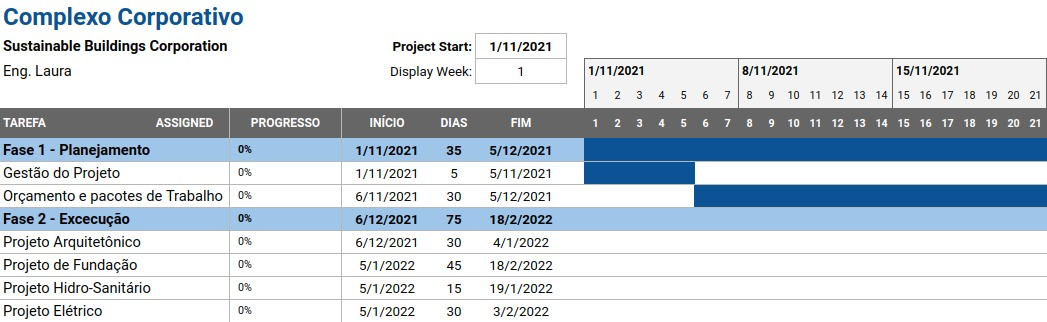
\includegraphics[scale=0.4]{fig/projeto.jpeg}
    \centering
    \caption{Cronograma do projeto.}
    \label{fig:cronograma}
\end{figure}

A folga de 10 dias no cronograma pode ser utilizado para que Laura consiga planejar e executar ações contra possíveis riscos ao projeto. Um dos riscos já mapeados antes do início das tarefas, são as férias de um membro importante da equipe. Para este caso em questão, Laura poderá movimentar as férias deste profissional para o início ou final do projeto, ou até mesmo trazer um auxiliar para acompanhar este profissional, deste modo, o auxiliar estará preparado para realizar as tarefas na ausência do membro da equipe. Ainda considerando possíveis riscos ao projeto, Laura deverá manter uma cadeia secundária de fornecedores, para rápida substituição em caso de falha na cadeia de fornecedores primária. Por fim, Laura também poderá mapear uma linha secundária de profissionais, para caso algum membro do time necessite se ausentar durante os 120 dias de projeto.

É importante salientar que, neste projeto, Laura fez uso de uma planilha específica para Gestão de Projetos. Entretanto, existem diversas ferramentas de mercado, gratuitas e pagas, que auxiliam a execução de projetos das mais diversas naturezas e escopos. Além disso, Laura optou por utilizar a metodologia Kanban \cite{arbulu2003kanban} na execução deste projeto. Além de Kanban, a equipe também adotará a \textit{daily} como uma cerimônia recorrente. Deste modo o time sempre estará alinhado sobre as demandas que estão acontecendo no projeto. Por fim, Laura também acredita que manter o time em sintonia é fundamental para o sucesso de uma grande entrega. Por este motivo, Laura adotou a cultura de celebrar com a equipe após a entrega de grandes marcos do projeto.

Conforme apresentado no case em questão, Laura usou de estratégias e artifícios para maximizar o cronograma proposto. Além disso, Laura também acredita em seus liderados, e que toda entrega é feita por pessoas. Laura está pronta para novos desafios.
% 